%% NOTE: this is the ORIGINAL LaTeX source and its "Normalization" section
%% argues the case *train with all K clusters active, evaluate with 1*, which is
%% the REVERSE of what the code does (and of Algorithm 5 in this same document).
%% The corrected version lives in docs/METHOD.md. Fix this before compiling.

\documentclass[11pt,a4paper]{article}

% Packages
\usepackage[utf8]{inputenc}
\usepackage[margin=1in]{geometry}
\usepackage{amsmath,amssymb,amsthm}
\usepackage{graphicx}
\usepackage{hyperref}
\usepackage{listings}
\usepackage{xcolor}
\usepackage{algorithm}
\usepackage{algpseudocode}
\usepackage{booktabs}
\usepackage{tikz}
\usetikzlibrary{shapes,arrows,positioning}

% Code listing settings
\lstset{
    language=Python,
    basicstyle=\ttfamily\small,
    keywordstyle=\color{blue},
    commentstyle=\color{gray},
    stringstyle=\color{red},
    showstringspaces=false,
    breaklines=true,
    frame=single,
    numbers=left,
    numberstyle=\tiny\color{gray}
}

% Custom commands
\newcommand{\R}{\mathbb{R}}
\newcommand{\argmax}{\operatorname{argmax}}
\newcommand{\softmax}{\operatorname{softmax}}

% Title
\title{\textbf{Ensemble Federated Learning:\\Complete Technical Explanation}}
\author{Technical Documentation}
\date{\today}

\begin{document}

\maketitle

\begin{abstract}
This document provides a comprehensive technical explanation of the Ensemble Federated Learning method, including detailed mathematical formulations, architecture descriptions, forward pass mechanics, normalization strategies, and implementation details. The ensemble approach addresses data heterogeneity in federated learning by creating cluster-specific feature extractors while maintaining a shared classifier.
\end{abstract}

\tableofcontents
\newpage

\section{High-Level Overview}

The \textbf{Ensemble Federated Learning} method addresses data heterogeneity in federated learning through a hierarchical architecture consisting of:

\begin{enumerate}
    \item \textbf{Client clustering} based on gradient similarity patterns
    \item \textbf{Cluster-specific feature extractors} (one per cluster)
    \item \textbf{Shared global classifier} across all clients
    \item \textbf{Ensemble prediction} combining features from multiple models
\end{enumerate}

\subsection{Key Insight}

Traditional Federated Averaging (FedAvg) forces all clients to converge to a single global model, which performs poorly when clients have heterogeneous data distributions. The ensemble method recognizes that:

\begin{itemize}
    \item Clients with different data distributions require \textit{different feature extractors}
    \item All clients can still share a \textit{common classifier} for the final prediction task
\end{itemize}

\section{Architecture Components}

\subsection{ResNet Feature Extractor}

The feature extractor removes the final classification layer from ResNet18 and outputs a feature vector instead of class logits.

\begin{lstlisting}[caption={ResNet Feature Extractor Implementation}]
class ResNetFeatureExtractor(nn.Module):
    def __init__(self, original_model):
        super().__init__()
        self.features = nn.Sequential(
            original_model.conv1,
            original_model.bn1,
            original_model.relu,
            original_model.maxpool,
            original_model.layer1,
            original_model.layer2,
            original_model.layer3,
            original_model.layer4,
            original_model.avgpool
        )
    
    def forward(self, x):
        x = self.features(x)
        x = torch.flatten(x, 1)
        return x
\end{lstlisting}

\textbf{Input/Output:}
\begin{itemize}
    \item Input: $\mathbf{x} \in \R^{B \times 3 \times 32 \times 32}$ (batch of CIFAR-10 images)
    \item Output: $\mathbf{z} \in \R^{B \times 512}$ (feature vectors)
\end{itemize}

\subsection{Ensemble Model Architecture}

The ensemble model combines $K$ feature extractors with a shared classifier.

\begin{center}
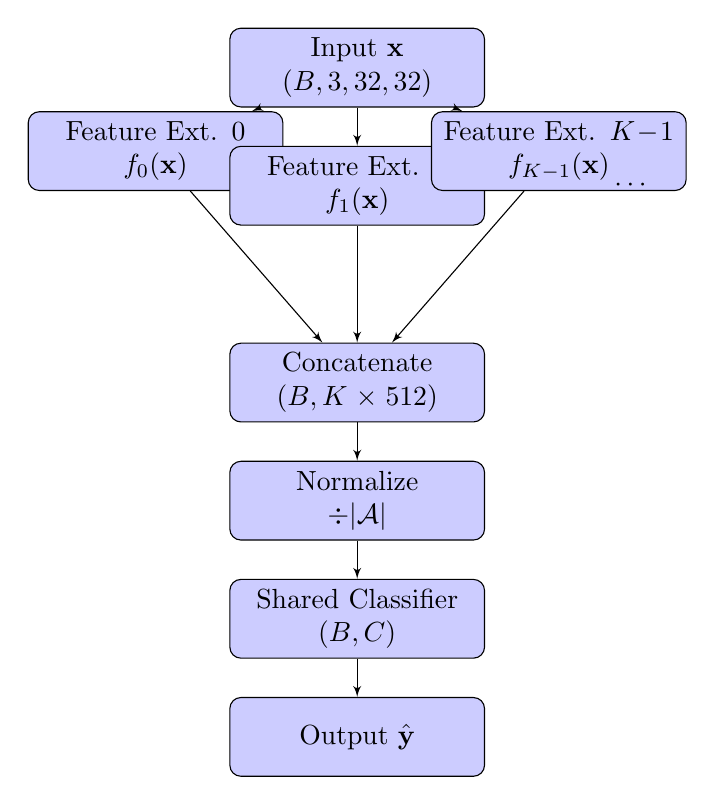
\begin{tikzpicture}[
    node distance=1.5cm,
    block/.style={rectangle, draw, fill=blue!20, text width=3cm, text centered, rounded corners, minimum height=1cm},
    line/.style={draw, -latex'}
]
    \node [block] (input) {Input $\mathbf{x}$\\$(B, 3, 32, 32)$};
    \node [block, below left of=input, xshift=-1.5cm] (f0) {Feature Ext. 0\\$f_0(\mathbf{x})$};
    \node [block, below of=input] (f1) {Feature Ext. 1\\$f_1(\mathbf{x})$};
    \node [block, below right of=input, xshift=1.5cm] (fk) {Feature Ext. $K\!-\!1$\\$f_{K-1}(\mathbf{x})$};
    \node [block, below of=f1, yshift=-1cm] (concat) {Concatenate\\$(B, K \times 512)$};
    \node [block, below of=concat] (norm) {Normalize\\$\div |\mathcal{A}|$};
    \node [block, below of=norm] (classifier) {Shared Classifier\\$(B, C)$};
    \node [block, below of=classifier] (output) {Output $\hat{\mathbf{y}}$};
    
    \path [line] (input) -- (f0);
    \path [line] (input) -- (f1);
    \path [line] (input) -- (fk);
    \path [line] (f0) -- (concat);
    \path [line] (f1) -- (concat);
    \path [line] (fk) -- (concat);
    \path [line] (concat) -- (norm);
    \path [line] (norm) -- (classifier);
    \path [line] (classifier) -- (output);
    
    \node [right of=f1, xshift=2cm] {$\cdots$};
\end{tikzpicture}
\end{center}

\section{Mathematical Formulation}

\subsection{Notation}

\begin{table}[h]
\centering
\begin{tabular}{@{}lll@{}}
\toprule
Symbol & Meaning & Dimension \\ \midrule
$\mathbf{x}$ & Input image & $(B, 3, 32, 32)$ \\
$K$ & Number of clusters & scalar \\
$d$ & Feature dimension & 512 (ResNet18) \\
$C$ & Number of classes & 10 (CIFAR-10) \\
$f_k(\cdot)$ & Feature extractor for cluster $k$ & $\R^{3 \times 32 \times 32} \to \R^d$ \\
$\mathbf{z}_k$ & Features from cluster $k$ & $(B, d)$ \\
$\mathbf{Z}$ & Concatenated features & $(B, K \times d)$ \\
$\mathcal{A}$ & Set of active cluster indices & $\subseteq \{0, 1, \ldots, K-1\}$ \\
$\mathbf{W}$ & Classifier weight matrix & $(C, K \times d)$ \\
$\mathbf{b}$ & Classifier bias vector & $(C,)$ \\
\bottomrule
\end{tabular}
\caption{Mathematical notation used throughout this document}
\end{table}

\subsection{Forward Pass}

The forward pass through the ensemble consists of five steps:

\begin{algorithm}
\caption{Ensemble Forward Pass}
\begin{algorithmic}[1]
\Require Input $\mathbf{x} \in \R^{B \times 3 \times 32 \times 32}$, Active indices $\mathcal{A} \subseteq \{0, \ldots, K-1\}$
\Ensure Output logits $\hat{\mathbf{y}} \in \R^{B \times C}$

\State \textbf{Step 1: Feature Extraction}
\For{$k = 0$ to $K-1$}
    \State $\mathbf{z}_k \gets f_k(\mathbf{x}) \quad \text{where } \mathbf{z}_k \in \R^{B \times d}$
\EndFor

\State \textbf{Step 2: Concatenation with Masking}
\State Initialize $\mathbf{Z} \gets \mathbf{0}_{B \times (K \cdot d)}$
\For{$k \in \mathcal{A}$}
    \State $\mathbf{Z}[:, k \cdot d : (k+1) \cdot d] \gets \mathbf{z}_k$
\EndFor

\State \textbf{Step 3: Normalization}
\State $\mathbf{Z}_{\text{norm}} \gets \mathbf{Z} / |\mathcal{A}|$

\State \textbf{Step 4: Classification}
\State $\hat{\mathbf{y}} \gets \mathbf{Z}_{\text{norm}} \mathbf{W}^T + \mathbf{b}$

\State \textbf{Step 5: Prediction}
\State $\text{predictions} \gets \argmax(\hat{\mathbf{y}}, \text{dim}=1)$

\State \Return $\hat{\mathbf{y}}$
\end{algorithmic}
\end{algorithm}

\subsection{Complete Mathematical Expression}

The ensemble prediction can be written compactly as:

\begin{equation}
\hat{\mathbf{y}} = \mathbf{W} \times \left(\frac{1}{|\mathcal{A}|} \times \text{Concat}\left[\mathbf{z}_k \text{ for } k \in \mathcal{A}, \mathbf{0} \text{ for } k \notin \mathcal{A}\right]\right) + \mathbf{b}
\end{equation}

where:
\begin{align}
\mathbf{z}_k &= f_k(\mathbf{x}) && \text{(feature extraction)} \\
\text{Concat}[\cdot] &: \R^{B \times d} \times \cdots \times \R^{B \times d} \to \R^{B \times (K \cdot d)} && \text{(concatenation)} \\
\frac{1}{|\mathcal{A}|} &\in \R && \text{(scalar normalization)} \\
\mathbf{W} &\in \R^{C \times (K \cdot d)}, \quad \mathbf{b} \in \R^C && \text{(learned parameters)}
\end{align}

\section{Forward Pass: Concrete Example}

Let us trace through a complete forward pass with specific numerical dimensions.

\subsection{Setup}

\begin{itemize}
    \item Batch size: $B = 2$
    \item Number of clusters: $K = 3$
    \item Feature dimension: $d = 512$
    \item Number of classes: $C = 10$
    \item Active clusters: $\mathcal{A} = \{0, 2\}$ (clusters 0 and 2 only)
\end{itemize}

\subsection{Step 1: Feature Extraction}

\begin{align}
\mathbf{x} &\in \R^{2 \times 3 \times 32 \times 32} && \text{(input images)} \\
\mathbf{z}_0 &= f_0(\mathbf{x}) \in \R^{2 \times 512} && \text{(cluster 0 features)} \\
\mathbf{z}_1 &= f_1(\mathbf{x}) \in \R^{2 \times 512} && \text{(cluster 1 features, inactive)} \\
\mathbf{z}_2 &= f_2(\mathbf{x}) \in \R^{2 \times 512} && \text{(cluster 2 features)}
\end{align}

\subsection{Step 2: Concatenation with Masking}

Initialize zero tensor:
\begin{equation}
\mathbf{Z} = \mathbf{0}_{2 \times 1536} \in \R^{2 \times (3 \times 512)}
\end{equation}

Fill active clusters:
\begin{align}
\mathbf{Z}[:, 0:512] &\gets \mathbf{z}_0 && \text{(cluster 0 active)} \\
\mathbf{Z}[:, 512:1024] &\gets \mathbf{0} && \text{(cluster 1 inactive)} \\
\mathbf{Z}[:, 1024:1536] &\gets \mathbf{z}_2 && \text{(cluster 2 active)}
\end{align}

Result: $\mathbf{Z} \in \R^{2 \times 1536}$ with structure:
\begin{equation}
\mathbf{Z} = \left[\mathbf{z}_0 \mid \mathbf{0}_{512} \mid \mathbf{z}_2\right]
\end{equation}

\subsection{Step 3: Normalization}

\begin{equation}
\mathbf{Z}_{\text{norm}} = \frac{\mathbf{Z}}{|\mathcal{A}|} = \frac{\mathbf{Z}}{2}
\end{equation}

This divides all features by the number of active clusters:
\begin{equation}
\mathbf{Z}_{\text{norm}} = \left[\frac{\mathbf{z}_0}{2} \mid \mathbf{0}_{512} \mid \frac{\mathbf{z}_2}{2}\right] \in \R^{2 \times 1536}
\end{equation}

\subsection{Step 4: Classification}

\begin{align}
\hat{\mathbf{y}} &= \mathbf{Z}_{\text{norm}} \mathbf{W}^T + \mathbf{b} \\
&= (2 \times 1536) \times (1536 \times 10) + (10,) \\
&\in \R^{2 \times 10}
\end{align}

The weight matrix $\mathbf{W} \in \R^{10 \times 1536}$ has structure:
\begin{equation}
\mathbf{W} = \begin{bmatrix}
\mathbf{w}_{0,0:511} & \mathbf{w}_{0,512:1023} & \mathbf{w}_{0,1024:1535} \\
\mathbf{w}_{1,0:511} & \mathbf{w}_{1,512:1023} & \mathbf{w}_{1,1024:1535} \\
\vdots & \vdots & \vdots \\
\mathbf{w}_{9,0:511} & \mathbf{w}_{9,512:1023} & \mathbf{w}_{9,1024:1535}
\end{bmatrix}
\end{equation}

where each column block corresponds to one cluster's contribution.

\subsection{Step 5: Prediction}

\begin{equation}
\text{predictions} = \argmax(\hat{\mathbf{y}}, \text{dim}=1) \in \{0, 1, \ldots, 9\}^2
\end{equation}

During training, we use the logits with cross-entropy loss:
\begin{equation}
\mathcal{L} = -\frac{1}{B} \sum_{i=1}^{B} \log \frac{\exp(\hat{y}_{i,c_i})}{\sum_{j=1}^{C} \exp(\hat{y}_{i,j})}
\end{equation}

where $c_i$ is the true class label for sample $i$.

\section{Normalization: Mathematical Analysis}

\subsection{Why Normalization is Critical}

The normalization step $\mathbf{Z} / |\mathcal{A}|$ is essential for maintaining consistent predictions across different numbers of active clusters.

\subsubsection{Problem Without Normalization}

Consider training with all $K$ clusters active:
\begin{equation}
\hat{\mathbf{y}}_{\text{train}} = \mathbf{W} \times \left[\mathbf{z}_0, \mathbf{z}_1, \ldots, \mathbf{z}_{K-1}\right] + \mathbf{b}
\end{equation}

The classifier weights $\mathbf{W}$ are optimized for this magnitude of features.

At inference with only 1 cluster active:
\begin{equation}
\hat{\mathbf{y}}_{\text{test}} = \mathbf{W} \times \left[\mathbf{z}_0, \mathbf{0}, \ldots, \mathbf{0}\right] + \mathbf{b}
\end{equation}

The logits will be approximately $\frac{1}{K}$ of the expected magnitude, severely affecting predictions.

\subsubsection{Solution: Normalization}

With normalization, we ensure magnitude consistency:

\textbf{Training (all $K$ active):}
\begin{equation}
\hat{\mathbf{y}}_{\text{train}} = \mathbf{W} \times \frac{\left[\mathbf{z}_0, \mathbf{z}_1, \ldots, \mathbf{z}_{K-1}\right]}{K} + \mathbf{b}
\end{equation}

\textbf{Inference (1 active):}
\begin{equation}
\hat{\mathbf{y}}_{\text{test}} = \mathbf{W} \times \frac{\left[\mathbf{z}_0, \mathbf{0}, \ldots, \mathbf{0}\right]}{1} + \mathbf{b}
\end{equation}

Now the effective feature magnitude is comparable in both cases.

\subsection{Interpretation: Averaging vs. Summing}

Normalization implements \textit{averaging} of features rather than \textit{summing}:

\begin{align}
\text{Sum:} \quad &\mathbf{z}_{\text{sum}} = \mathbf{z}_0 + \mathbf{z}_1 + \cdots + \mathbf{z}_{K-1} \\
\text{Average:} \quad &\mathbf{z}_{\text{avg}} = \frac{1}{K}\left(\mathbf{z}_0 + \mathbf{z}_1 + \cdots + \mathbf{z}_{K-1}\right)
\end{align}

Averaging ensures:
\begin{itemize}
    \item Magnitude is independent of $|\mathcal{A}|$
    \item Predictions are consistent across different active cluster counts
    \item Each cluster contributes equally on average
\end{itemize}

\subsection{Impact on Gradient Flow}

During backpropagation, the normalization affects gradients:

\begin{align}
\frac{\partial \mathcal{L}}{\partial \mathbf{z}_k} &= \frac{\partial \mathcal{L}}{\partial \hat{\mathbf{y}}} \times \frac{\partial \hat{\mathbf{y}}}{\partial \mathbf{Z}_{\text{norm}}} \times \frac{\partial \mathbf{Z}_{\text{norm}}}{\partial \mathbf{z}_k} \\
&= \frac{\partial \mathcal{L}}{\partial \hat{\mathbf{y}}} \times \mathbf{W}^T \times \frac{1}{|\mathcal{A}|}
\end{align}

The gradient is scaled by $\frac{1}{|\mathcal{A}|}$, ensuring balanced learning regardless of how many clusters are active during training.

\section{Training Phases}

\subsection{Phase 1: Warmup}

\textbf{Objective:} Train initial models and collect gradient information for clustering.

\begin{algorithm}
\caption{Warmup Phase (Single Client Finetuning)}
\begin{algorithmic}[1]
\Require Global model $f_{\text{global}}$, Training subsets $\{\mathcal{D}_i\}_{i=1}^N$
\Ensure Gradient collection $\{\mathbf{g}_i\}_{i=1}^N$

\For{$i = 1$ to $N$} \Comment{For each client}
    \State Initialize $f_i \gets f_{\text{global}}$ \Comment{Local model}
    \For{epoch $= 1$ to $E_{\text{warmup}}$}
        \State $\mathbf{g}_{\text{epoch}} \gets \mathbf{0}$ \Comment{Accumulator}
        \State $n_{\text{batches}} \gets 0$
        \For{batch $(\mathbf{x}, \mathbf{y}) \in \mathcal{D}_i$}
            \State $\hat{\mathbf{y}} \gets f_i(\mathbf{x})$
            \State $\mathcal{L} \gets \text{CrossEntropy}(\hat{\mathbf{y}}, \mathbf{y})$
            \State Compute $\nabla \mathcal{L}$ via backpropagation
            \State Extract $\nabla_{\text{layer4+fc}} \gets$ gradients from layer4 and fc
            \State $\mathbf{g}_{\text{epoch}} \gets \mathbf{g}_{\text{epoch}} + \text{flatten}(\nabla_{\text{layer4+fc}})$
            \State Update $f_i$ using optimizer
            \State $n_{\text{batches}} \gets n_{\text{batches}} + 1$
        \EndFor
        \State Store $\mathbf{g}_i[\text{epoch}] \gets \mathbf{g}_{\text{epoch}} / n_{\text{batches}}$
    \EndFor
\EndFor
\State \Return $\{\mathbf{g}_i\}_{i=1}^N$ \Comment{Gradients for clustering}
\end{algorithmic}
\end{algorithm}

\textbf{Gradient Extraction:} For each client, we extract and concatenate gradients from:
\begin{itemize}
    \item \textbf{layer4}: High-level feature representations (sensitive to data distribution)
    \item \textbf{fc}: Task-specific layer (captures label distribution differences)
\end{itemize}

\subsection{Phase 2: Clustering}

\textbf{Objective:} Group clients with similar data distributions based on gradient patterns.

\begin{algorithm}
\caption{Client Clustering}
\begin{algorithmic}[1]
\Require Gradients $\{\mathbf{g}_i\}_{i=1}^N$, Number of clusters $K$
\Ensure Cluster assignments $\{\kappa_i\}_{i=1}^N$ where $\kappa_i \in \{0, \ldots, K-1\}$

\State \textbf{Step 1: Average gradients across epochs}
\For{$i = 1$ to $N$}
    \State $\bar{\mathbf{g}}_i \gets \frac{1}{E_{\text{warmup}}} \sum_{\text{epoch}=1}^{E_{\text{warmup}}} \mathbf{g}_i[\text{epoch}]$
\EndFor

\State \textbf{Step 2: Center the gradient matrix}
\State $\boldsymbol{\mu} \gets \frac{1}{N} \sum_{i=1}^{N} \bar{\mathbf{g}}_i$ \Comment{Mean gradient}
\For{$i = 1$ to $N$}
    \State $\Delta\mathbf{g}_i \gets \bar{\mathbf{g}}_i - \boldsymbol{\mu}$
\EndFor

\State \textbf{Step 3: Normalize to unit length}
\For{$i = 1$ to $N$}
    \State $\tilde{\mathbf{g}}_i \gets \frac{\Delta\mathbf{g}_i}{\|\Delta\mathbf{g}_i\|_2 + \epsilon}$
\EndFor

\State \textbf{Step 4: K-Means clustering}
\State $\{\kappa_i\}_{i=1}^N \gets \text{KMeans}(\{\tilde{\mathbf{g}}_i\}_{i=1}^N, K)$

\State \Return $\{\kappa_i\}_{i=1}^N$
\end{algorithmic}
\end{algorithm}

\textbf{K-Means Objective:}
\begin{equation}
\min_{\{\boldsymbol{\mu}_k\}_{k=0}^{K-1}} \sum_{k=0}^{K-1} \sum_{i: \kappa_i = k} \|\tilde{\mathbf{g}}_i - \boldsymbol{\mu}_k\|_2^2
\end{equation}

where $\boldsymbol{\mu}_k$ is the centroid of cluster $k$.

\subsection{Phase 3: Ensemble Initialization}

\textbf{Objective:} Create $K$ feature extractors and expand the classifier to accept concatenated features.

\begin{algorithm}
\caption{Ensemble Initialization}
\begin{algorithmic}[1]
\Require Global model $f_{\text{global}}$, Number of clusters $K$
\Ensure Feature extractors $\{f_k\}_{k=0}^{K-1}$, Classifier $g$

\State \textbf{Step 1: Create feature extractors}
\State $f_{\text{base}} \gets \text{ResNetFeatureExtractor}(f_{\text{global}})$
\For{$k = 0$ to $K-1$}
    \State $f_k \gets \text{DeepCopy}(f_{\text{base}})$
\EndFor

\State \textbf{Step 2: Expand classifier}
\State $\mathbf{W}_{\text{old}} \gets f_{\text{global}}.\text{fc.weight}$ \Comment{Shape: $(C, d)$}
\State $\mathbf{b}_{\text{old}} \gets f_{\text{global}}.\text{fc.bias}$ \Comment{Shape: $(C,)$}
\State Initialize $\mathbf{W}_{\text{new}} \in \R^{C \times (K \cdot d)}$, $\mathbf{b}_{\text{new}} \in \R^C$
\For{$k = 0$ to $K-1$}
    \State $\mathbf{W}_{\text{new}}[:, k \cdot d : (k+1) \cdot d] \gets \mathbf{W}_{\text{old}}$
\EndFor
\State $\mathbf{b}_{\text{new}} \gets \mathbf{b}_{\text{old}}$
\State $g \gets \text{Linear}(\mathbf{W}_{\text{new}}, \mathbf{b}_{\text{new}})$

\State \Return $\{f_k\}_{k=0}^{K-1}$, $g$
\end{algorithmic}
\end{algorithm}

\textbf{Weight Replication Rationale:} Copying the original weights $K$ times ensures the ensemble starts with the same prediction capacity as the warmup model. During training, the weight sections will diverge to specialize for each cluster.

\subsection{Phase 4: Hierarchical Training}

\textbf{Objective:} Train cluster-specific feature extractors while maintaining a shared classifier.

\subsubsection{Pooled Training (Notebook Implementation)}

\begin{algorithm}
\caption{Hierarchical Training (Pooled)}
\begin{algorithmic}[1]
\Require Feature extractors $\{f_k\}_{k=0}^{K-1}$, Classifier $g$, Training data $\{\mathcal{D}_i\}_{i=1}^N$, Cluster assignments $\{\kappa_i\}_{i=1}^N$
\Ensure Trained ensemble model

\For{round $= 1$ to $R$} \Comment{Training rounds}
    \For{$k = 0$ to $K-1$} \Comment{For each cluster}
        \State $\mathcal{D}_k \gets \bigcup_{i: \kappa_i = k} \mathcal{D}_i$ \Comment{Pool cluster data}
        \For{epoch $= 1$ to $E_{\text{local}}$}
            \For{batch $(\mathbf{x}, \mathbf{y}) \in \mathcal{D}_k$}
                \State \textbf{Forward:}
                \State $\mathbf{z}_k \gets f_k(\mathbf{x})$
                \State $\mathbf{Z} \gets [\mathbf{0}, \ldots, \mathbf{z}_k, \ldots, \mathbf{0}]$ \Comment{Only cluster $k$ active}
                \State $\mathbf{Z}_{\text{norm}} \gets \mathbf{Z} / 1$ \Comment{Normalize by 1}
                \State $\hat{\mathbf{y}} \gets g(\mathbf{Z}_{\text{norm}})$
                \State $\mathcal{L} \gets \text{CrossEntropy}(\hat{\mathbf{y}}, \mathbf{y})$
                \State \textbf{Backward:}
                \State Compute gradients $\nabla_{f_k} \mathcal{L}$, $\nabla_g \mathcal{L}$
                \State Update $f_k$ and $g$ using optimizer
            \EndFor
        \EndFor
    \EndFor
    \State Evaluate ensemble on validation set
\EndFor
\State \Return $\{f_k\}_{k=0}^{K-1}$, $g$
\end{algorithmic}
\end{algorithm}

\section{Implementation Details}

\subsection{Feature Concatenation with Masking}

The implementation uses zero-padding for inactive clusters:

\begin{lstlisting}[caption={Feature Masking Implementation}]
# Initialize zero tensor
all_features = torch.zeros(
    batch_size, 
    num_clusters * feature_dim, 
    device=x.device
)

# Fill only active clusters
for idx in active_indices:
    features = self.models[idx](x)  # (B, 512)
    
    start_idx = idx * self.feature_dim
    end_idx = (idx + 1) * self.feature_dim
    all_features[:, start_idx:end_idx] = features
\end{lstlisting}

This approach:
\begin{itemize}
    \item Allows dynamic activation of any subset of clusters
    \item Maintains consistent input dimension to the classifier
    \item Simplifies implementation compared to variable-length concatenation
\end{itemize}

\subsection{Gradient Extraction During Warmup}

\begin{lstlisting}[caption={Gradient Extraction}]
# Accumulate gradients from layer4 and fc
current_batch_grad = []
for name, param in model.named_parameters():
    if param.grad is not None and \
       ('layer4' in name or 'fc' in name):
        current_batch_grad.append(param.grad.view(-1))

# Flatten to single vector
flat_batch_grad = torch.cat(current_batch_grad)
\end{lstlisting}

The flattening operation $\text{view}(-1)$ converts gradients of any shape into 1D vectors for clustering.

\subsection{Classifier Weight Initialization}

\begin{lstlisting}[caption={Weight Expansion}]
old_fc = global_model.fc  # (C, d)
new_fc = nn.Linear(K * d, C)  # (C, K*d)

with torch.no_grad():
    for k in range(K):
        start = k * feature_dim
        end = (k + 1) * feature_dim
        new_fc.weight[:, start:end] = old_fc.weight
    
    new_fc.bias.copy_(old_fc.bias)
\end{lstlisting}

This ensures the ensemble starts with equivalent capacity to the original model.

\section{Summary and Advantages}

\subsection{Architecture Summary}

The ensemble method combines:
\begin{itemize}
    \item \textbf{$K$ feature extractors}: Cluster-specific, trained on similar data
    \item \textbf{1 shared classifier}: Global knowledge aggregation
    \item \textbf{Normalization}: Consistent predictions across active cluster counts
\end{itemize}

\subsection{Mathematical Summary}

\begin{equation}
\hat{\mathbf{y}} = \softmax\left(\mathbf{W} \times \left(\frac{1}{|\mathcal{A}|} \times \text{Concat}[\mathbf{z}_k \text{ for } k \in \mathcal{A}]\right) + \mathbf{b}\right)
\end{equation}

where $\mathbf{z}_k = f_k(\mathbf{x})$ are cluster-specific features.

\subsection{Key Advantages}

\begin{enumerate}
    \item \textbf{Handles heterogeneity}: Different feature extractors adapt to different data distributions
    \item \textbf{Shared knowledge}: Classifier benefits from all clients' data
    \item \textbf{Flexible inference}: Can evaluate with 1, some, or all clusters
    \item \textbf{Superior to FedAvg}: Avoids forcing a single model to fit heterogeneous data
\end{enumerate}

\subsection{Comparison with FedAvg}

\begin{table}[h]
\centering
\begin{tabular}{@{}lll@{}}
\toprule
Aspect & FedAvg & Ensemble Method \\ \midrule
Feature Extraction & Single shared model & $K$ cluster-specific models \\
Classifier & Single shared & Single shared \\
Data Heterogeneity & Poor performance & Robust \\
Inference Cost & Low & Medium ($K$ forward passes) \\
Communication Cost & Low & Medium (update $K$ models) \\
Accuracy on Non-IID & Moderate & High \\
\bottomrule
\end{tabular}
\caption{Comparison between FedAvg and Ensemble Federated Learning}
\end{table}

\section{References}

\begin{itemize}
    \item Implementation: \texttt{training/ensemble\_model.py}
    \item Federated training: \texttt{training/ensemble\_fl.py}
    \item Notebook: \texttt{experiments/ensemble\_dirichlet\_only.ipynb}
\end{itemize}

\end{document}
